\subsection{一致空间的伴随 Hausdorff 一致空间}

命题 16 设 X 是一致空间，i 是 X 到其 Hausdorff 完备化 \(\hat{\mathbf{X}}\) 中的典范映射。对 X 到 Hausdorff 一致空间 Y 中的每个一致连续映射 \(f\)，存在唯一的一致连续映射 \(h: i(\mathbf{X}) \to \mathbf{Y}\) 使 \(f = h \circ i\)。

我们可以把 Y 与其完备化 \(\hat{Y}\) 的一个子空间等同起来（第 7 目命题 12 的推论），于是 f 可看作 X 到 \(\hat{Y}\) 中的一致连续映射。由定理 3，f 这时具有形式 \(f = g \circ i\)，其中 g 是 \(\hat{X}\) 到 \(\hat{Y}\) 中的一致连续映射。若 h 是 g 在 \(i(X)\) 上的限制，则显然 \(f = h \circ i\)，且 h 把 \(i(X)\) 映到 Y 中。h 的唯一性是显然的。

因此，偶 \((i, i(X))\) 是某个泛映射问题（《集合论》，第四章，§ 3，第 1 目）的解，这次我们取 \(\Sigma\)-集为 Hausdorff 一致空间，取 \(\sigma\)-态射（相应地 \(\alpha\)-映射）为一致连续映射（相应地，X 到 Hausdorff 一致空间中的一致连续映射）。

定义 5 在定理 3 的证明中所定义的 Hausdorff 一致空间 \(i(\mathbf{X})\) 称为 \(\mathbf{X}\) 的伴随 Hausdorff 一致空间。

于是，X 的 Hausdorff 完备化就是 X 的伴随 Hausdorff 一致空间的完备化。

推论 设 X、Y 是两个一致空间，\(X'\)、\(Y'\) 是它们的伴随 Hausdorff 空间。对每个一致连续映射 \(f: X \to Y\)，存在唯一的一致连续映射 \(f': X' \to Y'\) 使图表

\pandocbounded{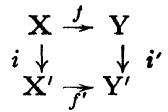
\includegraphics[keepaspectratio]{images/part002_3c8eaa6f.jpg}}

可交换，其中 \(i\) 与 \(i'\) 是典范映射。

对 \(i' \circ f: \mathbf{X} \to \mathbf{Y}'\) 应用命题 16。

一致空间的伴随 Hausdorff 空间也可以用下列性质来刻画：

命题 17 设 X 是一致空间，\(i(X)\) 是它的伴随 Hausdorff 空间，并设 \(f\) 是 X 到 Hausdorff 一致空间 \(X'\) 上的映射，使得 X 的一致结构是经由 \(f\) 从 \(X'\) 的一致结构取逆像而得的。则映射 \(g:i(X)\to X'\)（它使 \(f=g\circ i\)）是一个同构。

由命题 16，g 一致连续；g 显然是满射，并且也是单射，因为关系 \(f(x) = f(y)\) 按定义蕴含 \((x,y)\) 属于 X 的所有一致邻域，从而 \(i(x)=i(y)\)（第 7 目命题 12）。最后，\(X'\) 的一致邻域是 X 的一致邻域在 \(f\times f\) 下的像（§ 2 第 4 目的注），因而它们也是经由 \(g\times g\) 从 \(i(\mathbf{X})\) 的一致邻域得到的像（第 7 目命题 12）；由此即得结论。

注。设 R 是 X 上的等价关系 \(i(x) = i(x')\)。我们已看到（第 7 目命题 12），R 的图像 C 是 X 的所有一致邻域之交。显然，X 中的每个开集（因而每个闭集）关于 R 是饱和的；考虑到拓扑的逆像的定义，我们断言，商空间 X/R 到 \(i(X)\) 上的典范双射（由 \(i\) 所诱导）是一个同胚。因此，作为拓扑空间，X 的伴随 Hausdorff 空间可与 X/R 等同。典范映射 \(i: X \to i(X)\) 是开的和闭的，甚至是逆紧的（第一章 § 10 第 2 目的例）。

设 \(X'\) 是另一个一致空间，\(C'\) 是 \(X'\) 的所有一致邻域之交，\(R'\) 是以 \(C'\) 为图像的等价关系。设 \(f: X \to X'\) 是连续映射。由于在 \(f\) 之下，\(f(x)\) 的任一邻域的逆像是 \(x\) 的邻域，可知在 \(f\) 之下 \(C'(f(x))\) 的逆像包含 \(C(x)\)，因此 \(f\) 与 \(R\) 及 \(R'\) 相容，并诱导出一个连续映射 \(X/R \to X'/R'\)（第一章 § 3 第 4 目命题 6 的推论）。这推广了命题 16 的推论。

